/F30/ \\ \\
Prozess: Mitglieder in eine Gruppe einladen\\
Ziel: Mitglieder erhalten einen Link zur Gruppe\\
Kategorie: primär\\
Vorbedingung: Gruppe wurde bereits erstellt\\
Nachbedingung (Erfolg): zukünftige Gruppenmitglieder erhalten einen Link\\
Nachbedingung (Fehlschlag): zukünftige Gruppenmitglieder erhalten keinen Link\\
Akteure: Gruppenadministrator\\
Auslösendes Ereignis: Ein oder mehrere Personen sind noch nicht Mitglieder der Gruppe\\
Beschreibung:\\
1.) Gruppenadministrator macht sich Gedanken welche Personen er in die Gruppe einladen möchte\\
2.) Er tippt auf den Namen der Gruppe und sieht die allgemeinen Informationen über die Gruppe (Namen, Mitglieder)\\
3.) Über "Share Link" kann er auswählen, über welchen externen Messenger er den Link weiterleiten möchte\\
4.) Er wählt den gewünschten Messenger und seine Kontakte und bestätigt\\
5.) Link wird an die ausgewählten Kontakte versendet\\ \\
/F40/ Prozess: Treffpunkt (Ort/Zeit) festlegen (Admin)\\
Ziel: Mitglieder erhalten definitive Angaben für den nächsten Termin\\
Kategorie: primär\\
Vorbedingung: feste Gruppe existiert, Mitglieder sind bestimmt, Administrator ist festgelegt\\
Nachbedingung (Erfolg): Alle Mitglieder können sehen, wann und wo (optional) das nächste Treffen stattfinden wird\\
Nachbedingung (Fehlschlag): Gruppenmitglied bekommt keine Einsicht zu den Daten des nächsten Treffens\\
Akteure: Gruppenadministrator\\
Auslösendes Ereignis: Ein neues Treffen ist in Planung\\
1.) Gruppenadministrator macht sich Gedanken, wann und wo das nächste Treffen der Gruppe stattfinden soll\\
2.) Er tippt auf den Namen der Gruppe und sieht die allgemeinen Informationen über die Gruppe (Namen, Mitglieder)\\
3.) Er tippt auf den Button "Ereignis erstellen"\\
4.) Er wird weitergeleitet zu einem neuen Fenster, in dem er aufgefordert wird Zeit und vorläufigen Treffpunkt des nächsten Treffens einzugeben\\
5.) nach Eingabe von mindestens einem der beiden Parameter, kann er das neue Treffen über einen Button "Treffen bestätigen" bestätigen\\
6.) nach Bestätigung des Treffens, wird ihm angezeigt\\
6.a) ob das Erstellen des neuen Treffens erfolgreich war
6.b) oder ob das Erstellen des neuen Treffens nicht erfolgreich war.
7.a) war das Erstellen des neuen Treffens erfolgreich, so wird er zurück geleitet auf die Gruppe und bekommt nun, wie alle Gruppenmitglieder die auf die Gruppe tippen, zusätzlich zu Namen und Mitglieder das neue Treffen angezeigt, das mit Zeit und Treffpunkt zu sehen ist\\
7.b) war das Erstellen des neuen Treffens nicht erfolgreich, so wird ihm in einem kleinen Fenster im Vordergrund angezeigt, welcher Fehler aufgetreten ist und er wird zur erneuten Eingabe aufgefordert. Durch drücken des Buttons "okay" wird das kleine Fenster geschlossen und er kommt zurück zu Punkt 4)\\ \\
/F50/ Prozess: Gruppe verlassen\\
Ziel: ein Mitglied verlässt eine aktive Gruppe\\
Kategorie: primär
Vorbedingung: User ist Mitglied in einer aktiven Gruppe
Nachbedingung (Erfolg): User ist kein Mitglied mehr der aktiven Gruppe\\
Nachbedingung (Fehlschlag): User ist weiterhin Mitglied der aktiven Gruppe\\
Akteure: Gruppenmitglied
Auslösendes Ereignis: User möchte aus einer aktiven Gruppe austreten\\
1.) User entscheidet sich, aus der Gruppe auszutreten\\
2.) Er tippt auf den Namen der Gruppe und sieht die allgemeinen Informationen über die Gruppe (Namen, Mitglieder)\\
3.) Er tippt auf den Button "Gruppe verlassen"\\
4.) Ihm wird ein kleines Fenster im Vordergrund angezeigt, das ihn erneut fragt, ob er diese Gruppe wirklich verlassen will\\
5.a) Er tippt auf den Button "Ja, Gruppe verlassen"\\
5.b) Er tippt auf den Button "Nein, in der Gruppe bleiben"\\
6.a) Er wird zurück geleitet auf die Startansicht mit der Übersicht über die Gruppen. Dabei ist die gelöschte Gruppe nicht mehr mit aufgelistet.\\
6.b) Das kleine Fenster wird geschlossen und er kommt zurück zu Punkt 2)\\
7.a) Bei allen weiteren Gruppenmitgliedern wird der Name dieses Users nicht mehr in der Liste der Gruppenmitglieder aufgeführt\\

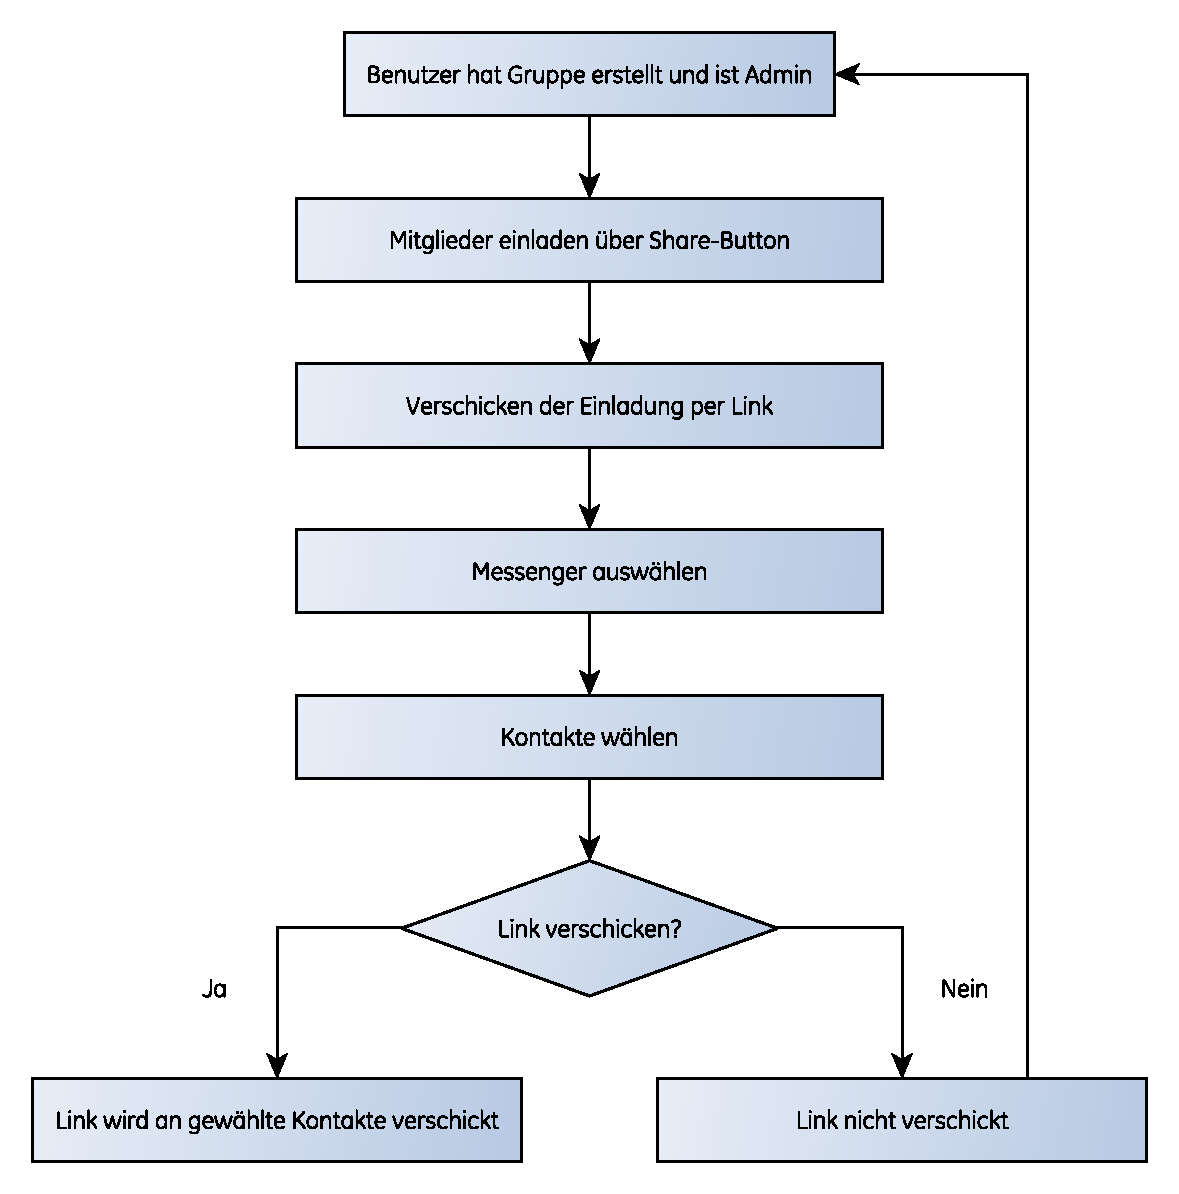
\includegraphics[scale=0.8]{./res/F30_mitglieder_einladen_flowgraph.pdf}
